\documentclass[tikz,border=7pt]{standalone}
\usepackage[T1]{fontenc}
\usepackage{lmodern}
\usepackage{helvet}
\renewcommand{\familydefault}{\sfdefault}
\usepackage[table]{xcolor}
\usepackage{tikz}
\usetikzlibrary{arrows.meta,positioning,calc}
\definecolor{ink}{HTML}{163B60}
\definecolor{wash}{HTML}{E4F1FC}
\tikzset{box/.style={draw=ink,rounded corners=3pt,line width=.8pt,minimum height=1cm,align=center,inner sep=8pt},flow/.style={-{Stealth[length=2.5mm]},draw=ink,line width=1pt},font=\sffamily\normalsize,every node/.style={text=ink}}
\begin{document}
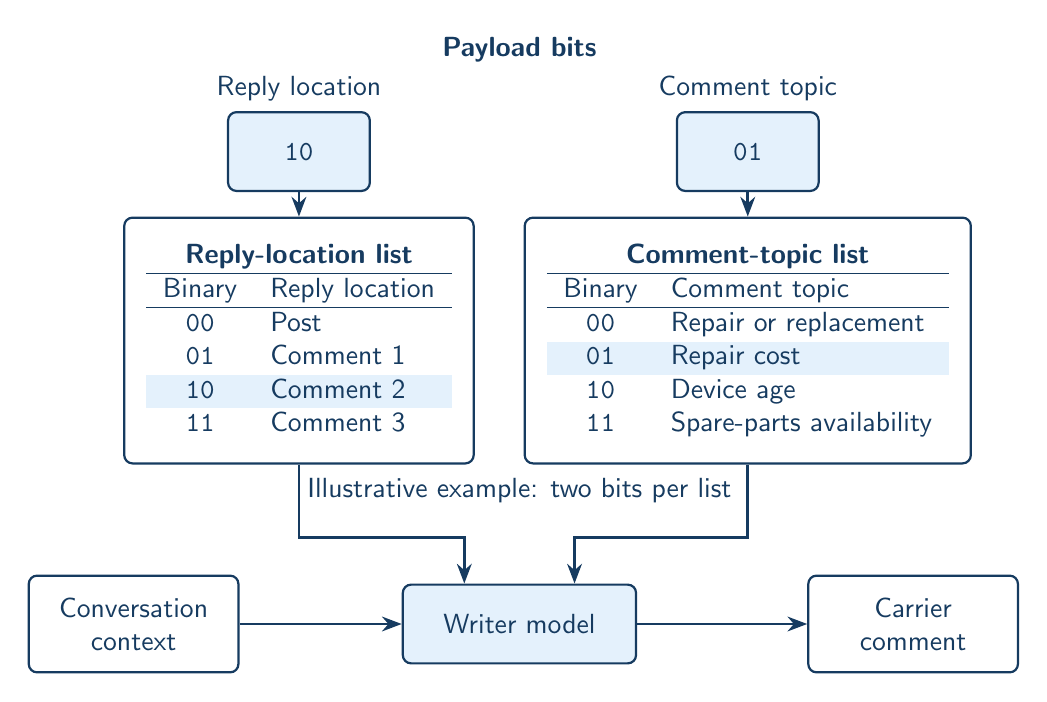
\begin{tikzpicture}
\node at (5.5,5.3) {\textbf{Payload bits}};
\node[box,fill=wash,minimum width=1.8cm] (parentbits) at (2.7,4) {\texttt{10}};
\node[anchor=south] at (parentbits.north) {Reply location};
\node[box,fill=wash,minimum width=1.8cm] (topicbits) at (8.4,4) {\texttt{01}};
\node[anchor=south] at (topicbits.north) {Comment topic};
\node[box] (parents) at (2.7,1.6) {\begin{tabular}{cl}\multicolumn{2}{c}{\textbf{Reply-location list}}\\\hline
Binary & Reply location\\\hline
\texttt{00} & Post\\
\texttt{01} & Comment 1\\
\rowcolor{wash}\texttt{10} & Comment 2\\
\texttt{11} & Comment 3
\end{tabular}};
\node[box] (topics) at (8.4,1.6) {\begin{tabular}{cl}\multicolumn{2}{c}{\textbf{Comment-topic list}}\\\hline
Binary & Comment topic\\\hline
\texttt{00} & Repair or replacement\\
\rowcolor{wash}\texttt{01} & Repair cost\\
\texttt{10} & Device age\\
\texttt{11} & Spare-parts availability
\end{tabular}};
\draw[flow] (parentbits) -- (parents);
\draw[flow] (topicbits) -- (topics);
\node[fill=white,inner sep=3pt] at (5.5,-.3) {Illustrative example: two bits per list};
\node[box,fill=wash,text width=2.4cm] (writer) at (5.5,-2) {Writer model};
\node[box,text width=2.1cm] (context) at (0.6,-2) {Conversation\\context};
\node[box,text width=2.1cm] (output) at (10.5,-2) {Carrier\\comment};
\draw[flow] (parents.south) -- (2.7,-.9) -| ([xshift=-.7cm]writer.north);
\draw[flow] (topics.south) -- (8.4,-.9) -| ([xshift=.7cm]writer.north);
\draw[flow] (context) -- (writer);
\draw[flow] (writer) -- (output);
\end{tikzpicture}
\end{document}
